\documentclass[conference]{IEEEtran}
\IEEEoverridecommandlockouts
% The preceding line is only needed to identify funding in the first footnote. If that is unneeded, please comment it out.
\usepackage{cite}
\usepackage{amsmath,amssymb,amsfonts}
\usepackage{algorithmic}
\usepackage{graphicx}
\usepackage{textcomp}
\usepackage{xcolor}
\usepackage{hyperref}
\usepackage{float}
\def\BibTeX{{\rm B\kern-.05em{\sc i\kern-.025em b}\kern-.08em
    T\kern-.1667em\lower.7ex\hbox{E}\kern-.125emX}}
\begin{document}

\title{Dokumentation der Softwarearchitektur des Projekts Graphvio}


% Authoren	
\author{
	
	\IEEEauthorblockN{Kreussel Lukas}
	\IEEEauthorblockA{
		\textit{l.kreussel@oth-aw.de}\\
	}
	
	\and

	\IEEEauthorblockN{Ziegler Andreas}
	\IEEEauthorblockA{
		\textit{a.ziegler1@oth-aw.de}\\
	}
}

\maketitle

\begin{abstract}
In diesem technischem Report wird die Softwarearchitektur des Projekts 
Graphvio vorgestellt. Das Projekt wurde im Rahmen der Vorlesung Semantic 
Web Technologien (SWT) implementiert. Ziel der Implementierung ist es, 
Suchanfragen in einer Graphdatenbank auszuwerten und die Ergebnisse 
über eine Webapplikation darzustellen.
\end{abstract}

\begin{IEEEkeywords}
 Semantic Web, Graph Database, Web UI
\end{IEEEkeywords}

\section{Introduction}
Bei der Applikation Graphvio werden vorhandene Datensätze von Streaminganbietern wie 
Amazon Prime, Disney Plus, Netflix und Hulu in eine lokale Graphdatenbank abgelegt.
Auf den Graph können dann per Rest-Schnittstelle Suchanfragen angewendet werden, die Ergebnisse
im JSON-Format liefern. Die Interaktion des Anwenders mit der Applikation erfolgt dabei über eine Web-UI basierend auf dem 
React Webframework.

\section{Architektur Allgemein}
% TODO:
\begin{figure*}
    \centering
    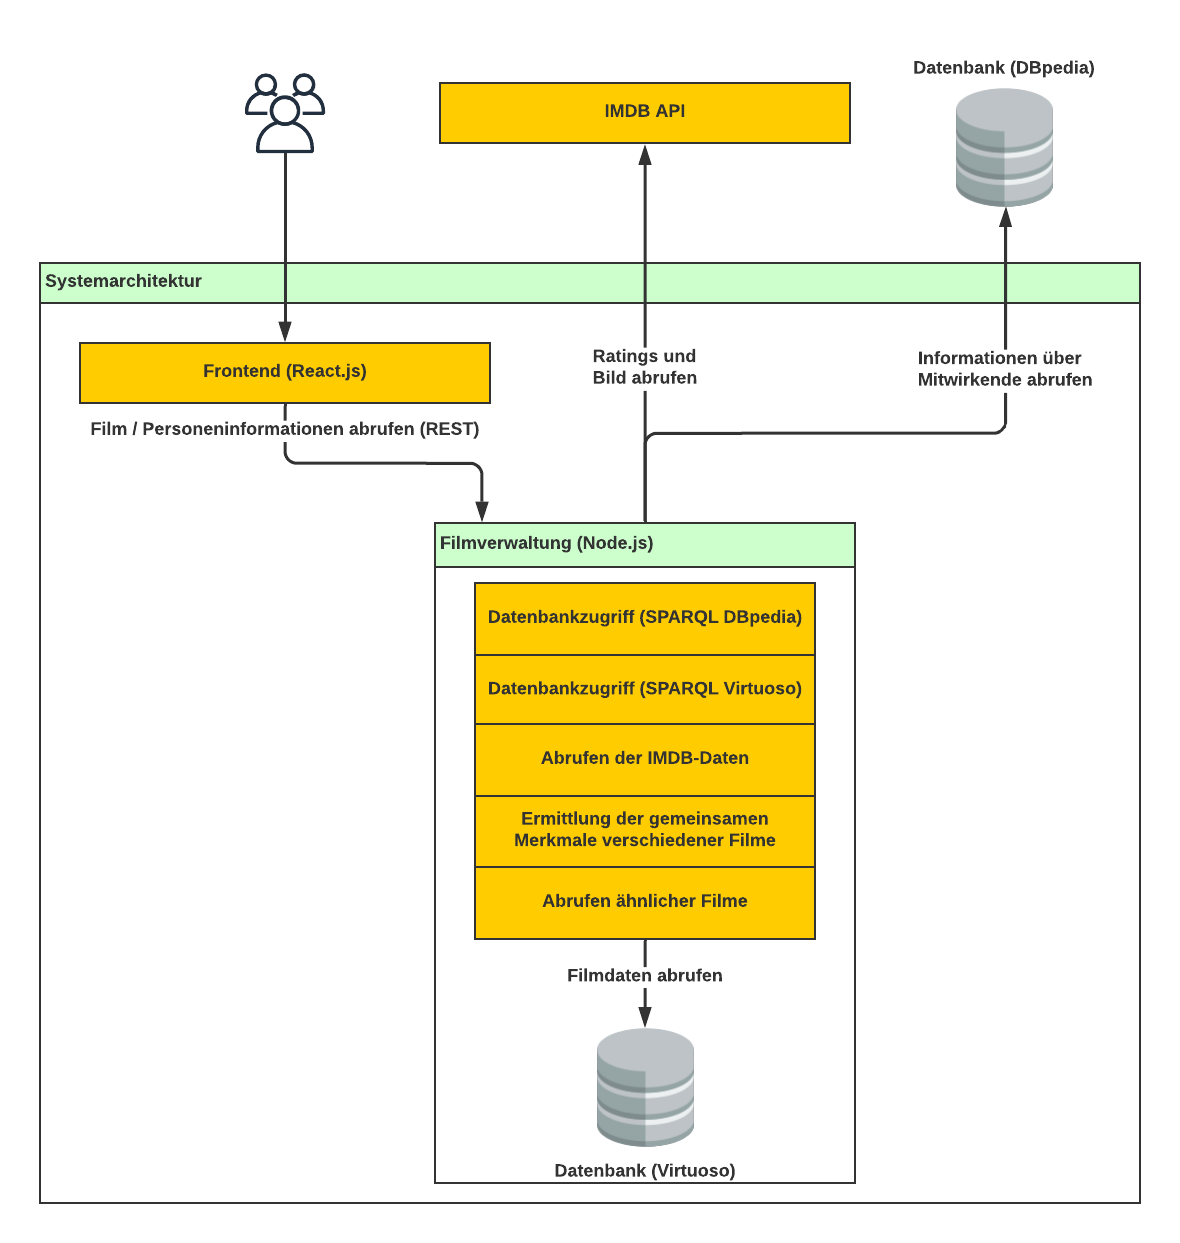
\includegraphics[width=\textwidth]{UebersichtGesamtsystem.png}
    \caption{Übersicht Gesamtsystem}
\end{figure*}

Als Architektur wird ein Ansatz verfolgt, der sich stark an Microservices orientiert.
Dadurch wird eine abgeschlossene Logik von Front- und Backendkomponenten erreicht, die jeweils
von einem Subteam entwickelt wird. Diese gekapselten Einheiten können jeweils als isolierte Applikation der Containervisualisierung
Docker betrieben werden. Durch eine zentrale Konfigurationsdatei des Containers können diese einfach zwischen den Teammitgliedern
ausgetauscht und ausgeführt werden. Damit wird eine hohe Portabilität gewährleistet.
Die Kommunikation der Teilsysteme wird durch eine sprachunabhängige REST-Schnittstelle angeboten. 
Dadurch wird es möglich einzelne Komponenten des Gesamtsystems auszutauschen, ohne größere Veränderungen an den anderen 
Microservices vornehmen zu müssen.
Dazu werden modulare Reactkomponenten erzeugt, die über Texteingaben und weitere Suchmaskenelemente Parameter der REST-Anfrage setzen.
Die zurückgelieferte Antwort der Anfrage im JSON-Format wird wiederum über modulare Reactkomponenten auf der Webapplikation dargestellt.\cite{microservices}

\section{Filmverwaltung}
% TODO:
Mithilfe des Web-Frameworks Express ist es möglich, Endpunkte für eine leistungsfähige API zu erstellen. Dabei
werden Client-Anfragen an passende Endpunkte des Node-Servers übergeben. Nach Bearbeitung dieser erfolgt eine Antwort
mit den Daten im JSON-Format. JSON ist ein Programmiersprachen unabhängiges Format, welches leicht lesbar ist, wenig Code erfordert
und zusätzlich schnell verarbeitet werden kann. Zusätzlich wird dabei wieder eine Austauschbarkeit einzelner Komponenten 
gefördert, da keine proprietären Datentypen verwendet werden müssen.
\\
\\
Die Funktionalität der Filmverwaltung umfasst folgende API-Zugriffe:
\smallskip

\textbf{Filmsuche (/db/search-movies)}
\begin{itemize}
\item Beschreibung:
    Bei der Filmsuche werden in der Datenbank passende Filme gesucht.
\item Parameter:
\begin{itemize}
    \item Teiltitel
    \item Provider
\end{itemize}
\item Rückgabe:
    Liste mit Filmen und deren Metadaten
\end{itemize}

\smallskip

\textbf{Personensuche (/db/search-persons)}
\begin{itemize}
\item Beschreibung:
    Bei der Personensuche werden in der DBpedia Daten zu Filmmitwirkenden eines Filmes gesucht.
\item Parameter:
    \begin{itemize}
    \item Filmtitel
    \item Erscheinungsjahr
    \end{itemize}
\item Rückgabe:
    Liste der Filmmitwirkenden und dazugehörigen Metadaten
\end{itemize}

\smallskip

\textbf{Gemeinsamkeitensuche (/db/compare-movies)}
\begin{itemize}
\item Beschreibung:
    Bei der Gemeinsamkeitensuche werden gemeinsame Merkmale einzelner Filme gesucht.
\item Parameter:
    Liste mit Filmtiteln
\item Rückgabe:
    Liste der Gemeinsamkeiten der Filme
\end{itemize}

\smallskip

\textbf{Suche nach ähnlichen Filmen (/db/search-similar-movies)}
\begin{itemize}
\item Beschreibung:
    Bei der Suche nach ähnlichen Filmen werden Filme gesucht, die Gemeinsamkeiten mit den angebegeben Filmen aufweisen.
\item Parameter:
    \begin{itemize}
    \item Liste mit Filmtiteln
    \item Streamingdienstanbieter der zu vergleichenden Filme
    \end{itemize}
\item Rückgabe:
    Liste mit Filmen
\end{itemize}

\smallskip

\textbf{Suche nach IMDB Daten eines Filmes (/imdb/search-imdbdata)}
\begin{itemize}
\item Beschreibung:
    Bei der Suche nach einem Film werden die Bewertungen und ein hinterlegtes Bild des Filmes in der IMDB gesucht.
\item Parameter:
    Titel des Filmes
\item Rückgabe:
    \begin{itemize}
    \item Liste mit Bewertungen des Filmes
    \item URL eines in der IMDB hinterlegten Bildes
    \end{itemize}
\end{itemize}

\smallskip

Die Verwaltung der Daten erfolgt mittels einer Virtuoso-Datenbank. Diese enthält Filmdaten der Streamingdienstanbieter
Netflix, Amazon-Prime, Disney+ und Hulu, welche aus Kaggle bezogen wurden.
Die Datensätze enthalten Filmtitel der jeweiligen Provider, sowie dessen Metainformationen wie 
Filmmitwirkende, Genre und Erscheinungsjahr. Mithilfe einer in Virtuoso angelegten View ist es möglich
mit SparQl-Statements auf die importierten Daten zu zugreifen.
\\
\\
Das Modul "Fetch SPARQL Endpoint" ermöglicht es innerhalb der Filmverwaltung eine Verbindung zwischen dem Node-Server
und der Virtuoso-Datenbank sowie der DBpedia aufzubauen. Anschließend können SPARQL-Statements abgesetzt und die Ergebnisse
asynchron Verarbeitet werden.
\\
\\
Die IMDB ist eine Datenbank zu Filmen, Fernsehserien, Videoproduktionen und Computerspielen sowie über Personen,
die daran mitgewirkt haben. Sie bietet eine API zum Zugriff auf diese Daten. Dafür wird ein API-Schlüssel benötigt, 
mit diesem sind täglich 100 Anfragen kostenfrei verfügbar. Nach überschreiten dieser Begrenzung sind keine weiteren Anfragen
an diesem Tag möglich, die Anfragenbegrenzung kann jedoch kostenpflichtig erhöht werden. 
\\
\\
Um die vorgesehene Funktionalität gewährleisten zu können, wurden mithilfe von Jest, einem JavaScript Testframework, 
Unit- und Integrationstests entworfen. Dadurch kann die interne Integrität, sowie die Anbindung an externe Systeme,
sichergestellt werden. Die Tests wurden dabei mit dem Arrange-Act-Assert-Pattern entworfen. Dieses soll eine 
übersichtliche Struktur und Einheitlichkeit garantieren.

\section{Frontend}

\subsection{Funktionalitäten Frontend}
Mit dem React Webframework ist das Frontend in der Programmiersprachen JavaScript erstellt, 
dazu wurde mithilfe von React Router Dom mehrere Seiten angelegt um die einzelnen Funktionalitäten breitzustellen. 
Auf der Startseite befinden sich zur erstmaligen Navigation mehrere Knöpfe, um zu den verschiedenen Funktionalitäten des Frontends weiterzuleiten.
Für die spätere Navigation wird auf jeder Seite eine Navigationleiste angezeigt, die folgende Weiterleitungen umfasst:

\begin{itemize}
    \item \textbf{Graphvio (/)}
    Mit einem Klick auf den Namen der Anwendung gelangt man zurück auf die Startseite, die auch beim ersten Aufruf der Seite angezeigt wird.
    \smallskip
    \item \textbf{Navigation} 
    In einem Dropdown können auf die einzelnen Funktionalitäten der Anwendung zugegriffen werden.
    \smallskip
    \subitem \textbf{Movie Search (/MovieSearchForm)}
    Auf dieser Seite kann in einem Textfeld der ganze Name eines Films oder ein Teil dessen Namens eigegeben werden und dieser wird in der Datenbank gesucht. 
    Die Ergebnisse werden in einer ausklappbaren Liste präsentiert, in der Informationen zu den einzelnen Filmen zu finden sind.
    \smallskip
    \subitem \textbf{Movie Compare (/MovieCompareSelect)}
    Die Movie Compare Seite akzeptiert in einem Textfeld mit Eingabeunterstützung mehrere Filme, welche verglichen werden sollen. 
    Daraufhin werden gemeinsame Merkmale der Filme, wie Genre, Direktor, Filmmitwirkende und Ursprungsland, angezeigt.
    \smallskip
    \subitem \textbf{Movie Recommend (/MovieRecommendForm)}
    Wie bei Movie Compare können hier mehrere Filme angebegeben werden. Aufgrund der gefundenen Gemeinsamkeiten werden hier ähnliche Filme aufgelistet, die in möglichst vielen Punkten mit den eigegebenen Filmen übereinstimmen. Die Ergebnisse werden in einer Liste wie bei der Filmsuche als ausklappbare Liste angezeigt. 
    \smallskip
    \item \textbf{About Us (/about-us)}
    Unter About Us sind Informationen zum Projekt und den beteiligten Personen zu finden.
\end{itemize}

Weiterhin besteht die Möglichkeit auf der Movie Search und Movie Recommend Seite in den Filmlisten über das \textbf{Cast} Feld der Film-Listeneinträge auf die  \textbf{Cast-Seite (/CastList)} zu wechseln, wo durch einen weiteren Datenbankaufruf mehr Informationen zu den Mitwirkenden zu finden. Falls dieser keine zusätzlichen Informationen findet wird dies dem Benutzer mitgeteilt, ansonsten werden die Mitwirkenden mit den erhaltenen Informationen in einer ausklappbaren Liste angezeigt.

\subsection{Aufbau Frontend}

Die einzelnen Seiteninhalte (Views) werden im Body der Seite gerendert 
und sind als modulare Elemente im Ordner View abgelegt. 
Die Ein- und Ausgabeelemente der einzelnen Views sind wiederum aus modularen Reactklassen aufgebaut.
Diese Klassen sind im Ordner Base abgelegt. Für die Umsetzung wurden sowohl reactspezifische als auch 
allgemeine HTML-Elemente verwendet.
Die formatspezifischen Eigenschaften dieser Elemente wurden in eigenen CSS-Dateien festgelegt.
Für die REST-Abfragen werden eigene Klassenfunktionen in den Views angelegt.
Die Aufrufe erfolgen dabei über das Package Axios.\cite{axios}
Das Package beinhaltet einen HTTP-Client, 
der asynchrone Aufrufe unterstützt und so das Rendering der Seite nicht negativ beeinflusst.

\subsection{Testing}
Zum Testen des Frontends wurden für Snapshot-Tests die React-Testing-Library\cite{reactTest} und für Funktionstest das Enzyme-Package\cite{enzyme} verwendet. 
Als TestRunner wurde die Jest-Library verwendet.

\begin{itemize}
    \item \textbf{Snapshot-Tests:}
    Die Snapshot-Tests erzeugen eine HTML-Document in welches die zu testende Komponente gerendert wird.
    Anschließend wird die HTML-Datei mit einer Snapshot-Datei verglichen, um sicher zu stellen das die Komponente wie erwartet dargestellt wird.
    \item \textbf{Funktionstest:}
    Bei den Funktionstests wird für jede Komponente eine Instanz mit dem Enzyme-Adapter erstellt.
    Mit dieser Objektinstanz könne verschieden Funktionen der Klasse getestet werden und geprüft werden ob Felder des Objekts richtig gesetzt werden.
\end{itemize}



\begin{thebibliography}{0}
	\bibitem{axios}Axios [Online] \url{https://www.npmjs.com/package/axios} (visited on Jan. 7, 2022)
    \bibitem{microservices}Microservice-Frontend-Architekturen [Online] \url{https://www.sigs-datacom.de/uploads/tx_dmjournals/attermeyer_OTS_Microservices_Docker_16.pdf} (visited on Jan. 7, 2022)
    \bibitem{reactTest}React-Testing [Online] \url{https://testing-library.com/docs/react-testing-library/intro/} (visited on Jan. 7, 2022)
    \bibitem{enzyme}Enzyme [Online] \url{https://www.npmjs.com/package/enzyme} (visited on Jan. 7, 2022)  
\end{thebibliography}

\end{document}
